\chapter{Descripción de la arquitectura de virtualización}

\lettrine[lines=1,slope=4pt,findent=0pt]{U}{}na vez introducido el vocabulario básico y tras haber indagado un poco más en la materia vamos a centrarnos en la arquitectura como tal.\\

\section{Tipos de Virtualización}
En el apartado anterior ya se pudo vislumbrar que existen diferentes formas de virtualización, y por ello, ahora vamos a nombrar todos los tipos y haremos, para cada uno, una pequeña descripción:

\subsection{Arquitectura del hipervisor}
El hipervisor permite la virtualización en el nivel de hardware en dispositivos sin sistema operativo, como CPU, memoria e interfaces de red. El software del hipervisor se ubica directamente entre el hardware físico y el sistema operativo. Este nivel de virtualización se denomina VMM or hipervisor.\\

El hipervisor proporciona hiperllamadas para los sistemas operativos y las aplicaciones invitadas. Los hipervisores pueden adoptar una arquitectura de micronúcleo, como en el ejemplo de Microsoft Hyper-V. También pueden tener una arquitectura monolítica, como por ejemplo VMware ESX para la virtualización de servidores.\\

Un hipervisor de micronúcleo solo incluye las funciones básicas e inmutables (como la administración de la memoria física y la programación de los procesadores). Los controladores de los dispositivos y los otros componentes mutables se encuentran fuera del hipervisor. Los hipervisores monolíticos implementan todas las funciones mencionadas, entre ellos los controladores de los dispositivos.\\

Por lo tanto, el tamaño del código del hipervisor es menor con un micronúcleo que en el caso monolítico. En esencia, el hipervisor debe ser capaz de convertir los dispositivos físicos en recursos virtuales disponibles para el uso de las máquinas virtuales.

\subsection{La arquitectura de Xen}
Xen es un hipervisor de código abierto desarrollado por la Universidad de Cambridge. Los componentes centrales de un sistema Xen son el hipervisor, el núcleo y las aplicaciones. La organización de estos tres componentes es muy importante.\\

Xen es un hipervisor de micronúcleo que separa las directivas de los mecanismos. El hipervisor de Xen implementa todos los mecanismos y deja que el Dominio 0 controle las directivas. No incluye ningún controlador en forma nativa. Solamente proporciona un mecanismo que permite que los sistemas operativos invitados tengan acceso directo a los dispositivos físicos.\\

Como resultado, el tamaño del hipervisor de Xen es bastante pequeño. Xen entrega un entorno virtual ubicado entre el hardware y el sistema operativo. Algunos proveedores desarrollan hipervisores comerciales para Xen; entre ellos Citrix XenServer y Oracle VM.\\

Al igual que los otros sistemas de virtualización, es posible ejecutar muchos sistemas operativos invitados encima del hipervisor. Sin embargo, no todos los sistemas operativos invitados se crean del mismo modo, y hay uno determinado que controla los demás. El sistema operativo invitado que tiene la capacidad de controlar se llama Dominio 0 y los otros se llaman Dominio U. El Dominio 0 es un invitado privilegiado de Xen. Es el primer dominio que se carga cuando Xen arranca, sin que estén disponibles los controladores del sistema de archivos. El Dominio 0 está diseñado para acceder directamente el hardware y administrar los dispositivos. Por lo tanto, una de las responsabilidades del Dominio 0 es asignar los recursos de hardware para los dominios invitados (los dominios del Dominio U).\\

Xen, por ejemplo, se basa en Linux y cumple con el nivel de seguridad de C2. La máquina virtual administrativa se llama Dominio 0 y tiene los privilegios necesarios para administrar las otras máquinas virtuales implementadas en el mismo host. Si se pierde la confidencialidad del Dominio 0 el hacker puede controlar todo el sistema.\\

Por lo tanto, el sistema de las máquinas virtuales necesita directivas de seguridad para mejorar la seguridad del Dominio 0. El Dominio 0, que se comporta como un VMM, permite que los usuarios creen, copien, guarden, lean, modifiquen, compartan, migren y reviertan las máquinas virtuales tan fácilmente como si se tratara de archivos. Por desgracia, esto también aporta problemas de seguridad durante el ciclo de vida del software y la vigencia de los datos.\\

Tradicionalmente, podríamos imaginar la vigencia de una máquina como una línea recta. El estado actual de la máquina es un punto que avanza en forma monotónica a medida que se ejecuta el software. Durante este tiempo, podemos hacer cambios en la configuración, instalar software y aplicar revisiones.\\

En este tipo de entorno, el estado de la máquina virtual es semejante a un árbol: en cualquier punto la ejecución puede moverse a N ramas diferentes, donde pueden existir varias instancias de una máquina virtual en cualquier punto de este árbol, en cualquier momento dado. Las máquinas virtuales tienen permiso de revertirse a estados previos de su ejecución (por ejemplo para corregir errores de configuración) o volver a ejecutarse del mismo punto varias veces (por ejemplo para distribuir contenidos dinámicos o circular una imagen de sistema “en vivo”).

\subsection{Traducción binaria en la virtualización completa}
Dependiendo de las tecnologías de la implementación, la virtualización del hardware se puede clasificar en dos categorías: la virtualización completa y la virtualización con un host.\\

La virtualización completa no tiene necesidad de modificar el sistema operativo host. Se vale de la traducción binaria para interceptar y virtualizar la ejecución de determinadas instrucciones confidenciales, y que no se pueden virtualizar. Los sistemas operativos invitados y sus aplicaciones consisten en instrucciones críticas y que no son críticas.\\

En un sistema con un host se usa un sistema operativo host y un sistema operativo invitado. Se construye una capa de software de virtualización entre los sistemas operativos host e invitado.\\

\subsection{Virtualización completa}
En la virtualización completa, las instrucciones que no son críticas se ejecutan directamente en el hardware, mientras que las instrucciones críticas se descubren y reemplazan con intercepciones en el VMM para emularlas en software. Tanto el método del hipervisor como el de VMM se consideran como virtualización completa.\\

¿Por qué solo las instrucciones críticas se interceptan en el VMM? Esto se debe a que la traducción binaria puede incurrir en una sobrecarga significativa en el rendimiento. Las instrucciones que no son críticas no controlan el hardware ni ponen en riesgo la seguridad del sistema, pero las instrucciones críticas sí lo hacen. Por lo tanto, al ejecutar las instrucciones que no son críticas en el hardware además de promover la eficiencia también protege el sistema.\\

Esta opción la implementó VMware y muchas otras empresas de software. El VMM examina el flujo de instrucciones e identifica las instrucciones privilegiadas críticas para el control y el comportamiento. Al identificar estas instrucciones, se interceptan en el VMM, que emula el comportamiento de estas instrucciones. El método que se emplea para la emulación se llama traducción binaria.\\

Por lo tanto la virtualización completa combina la traducción binaria con la ejecución directa. El sistema operativo invitado está totalmente desacoplado del hardware subyacente. Por consiguiente, el sistema operativo invitado desconoce que fue virtualizado.\\

Es probable que el rendimiento de la virtualización completa no sea ideal, ya que conlleva la traducción, que es un proceso bastante lento. La virtualización completa de aplicaciones que hace un uso extenso de los recursos de E/S es una tarea exigente. La traducción binaria emplea una caché de código para almacenar las instrucciones en caliente traducidas para mejorar el rendimiento, pero para esto tiene un costo en el consumo de memoria. El rendimiento de la virtualización completa en la arquitectura x86 normalmente es entre un 80 y un 97 porciento de la máquina host.

\subsection{Virtualización con un host}
Una arquitectura alternativa para la máquina virtual es instalar una capa de virtualización encima del sistema operativo host. Este sistema operativo host es responsable de administrar el hardware. Los sistemas operativos invitados se instalan encima del nivel de virtualización. Es posible ejecutar aplicaciones especializadas en las máquinas virtuales. También existen otras aplicaciones que se pueden ejecutar directamente con el sistema operativo host.\\

Esta arquitectura con un host tiene algunas ventajas marcadas. Primero, el usuario puede instalar esta arquitectura de máquina virtual sin modificar el sistema operativo host. El software de virtualización puede descansar en el sistema operativo host para entregar los controladores de dispositivos y otros servicios de bajo nivel. Esto simplifica el diseño de la máquina virtual y facilita la implementación.\\

Segundo, el método con un host es atractivo para muchas configuraciones de máquinas host. Comparado con la arquitectura de hypervisor o VMM, el rendimiento de la arquitectura con un host también puede ser bajo. Cuando una aplicación solicita acceso al hardware involucra cuatro niveles de asignación, lo que reduce el rendimiento significativamente. Cuando el Internet Security and Acceleration (ISA) de un sistema operativo invitado es diferente del ISA del hardware subyacente hay que realizar una traducción binaria. Aunque la arquitectura con un host es flexible, el rendimiento es demasiado lento para poder usarlo en la práctica.

\subsection{Paravirtualización}
La paravirtualización tiene que modificar el sistema operativo invitado. Una máquina virtual paravirtualizada proporciona API especiales que requieren de modificaciones considerables en las aplicaciones de usuario. La degradación del rendimiento es un problema fundamental de los sistemas virtualizados. Nadie quiere usar una máquina virtual que sea mucho más lenta que la máquina física.\\

El nivel de virtualización se puede insertar en diferentes lugares de la pila de software de la máquina. Pero la paravirtualización intenta reducir la sobrecarga de la virtualización y mejorar el rendimiento al modificar solo el núcleo del sistema operativo invitado. Al paravirtualizar los sistemas operativos invitados, reciben ayuda de un compilador inteligente que reemplaza las instrucciones del sistema operativo que no se pueden virtualizar con hiperllamadas.\\

El procesador x86 tradicional ofrece cuatro anillos de ejecución de instrucciones: Los Anillos 0, 1, 2 y 3. Cuanto menor el número del anillo, mayor el privilegio de la instrucción que se ejecuta. El sistema operativo es el responsable de administrar el hardware y las instrucciones privilegiadas que se ejecutan en el Anillo 0, mientras que las aplicaciones de usuario se ejecutan en el Anillo 3. El mejor ejemplo de la paravirtualización es Kernel-based Virtual Machine (KVM).\\

Al virtualizar el procesador x86 se inserta un nivel de virtualización entre el hardware y el sistema operativo. De acuerdo con la definición de los anillos de x86, el nivel de virtualización también se debiera instalar en el Anillo 0. Diferentes instrucciones en el Anillo 0 podrían causar algunos problemas. Pero cuando el núcleo del sistema operativo invitado se modifica para la virtualización ya no se puede ejecutar directamente en el hardware.\\

Aunque la paravirtualización reduce la sobrecarga, incurre en otros problemas. Primero, la compatibilidad y portabilidad se ponen en duda, ya que también tiene que funcionar con un sistema operativo que no ha sido modificado. Segundo, el costo de mantención de los sistemas operativos paravirtualizados es elevado, debido a que pueden requerir de cambios profundos en el núcleo del sistema operativo.\\

Finalmente, la ventajas de la paravirtualización en el rendimiento varían considerablemente debido a las variaciones en las cargas de trabajo. Comparada con la virtualización completa, la paravirtualización es relativamente fácil y más práctica. El problema principal de la virtualización completa es el rendimiento bajo de la traducción binaria. Es difícil acelerar la traducción binaria. Es por eso que muchos productos de virtualización tienen una arquitectura de paravirtualización. Los productos populares Xen, KVM y VMware ESX son buenos ejemplos de esto.\\

KVM es una herramienta de paravirtualización asistida por hardware que mejora el rendimiento y funciona con sistemas operativos sin modificar como Windows, Linux, Solaris y otras variantes de Unix.\\

Este es un sistema de paravirtualización de Linux; forma parte de la versión2.6.20 del núcleo de Linux. El núcleo existente de Linux lleva a cabo la administración de la memoria y las actividades de programación. KVM se encarga del resto, lo que lo hace más sencillo que el hipervisor, que controla toda la máquina.\\

A diferencia de la arquitectura de virtualización completa que intercepta y emula las instrucciones privilegiadas y confidenciales en tiempo de ejecución, la paravirtualización se encarga de estas instrucciones en tiempo de compilación. El núcleo del sistema operativo invitado se modifica para reemplazar las instrucciones privilegiadas y confidenciales con hiperllamadas al hipervisor o VMM. Xen es un ejemplo de esta arquitectura paravirtualizada.\\

Las instrucciones privilegiadas se implementan con hiperllamadas al hipervisor. Después de reemplazar las instrucciones con las hiperllamadas, el sistema operativo modificado emula el comportamiento del sistema operativo invitado original. En los sistemas Unix, las llamadas al sistema implican una interrupción o rutina de servicio. Las hiperllamadas aplican una rutina de servicio dedicada en Xen.\\

Los diferentes tipos de arquitecturas de virtualización tienen diferentes fortalezas y debilidades. Examine cada una y podrá aplicar la arquitectura más adecuada para su entorno.


\section{Componentes}

Como bien se ha introducido antes, en la arquitectura de hipervisor

\subsection{Máquina Virtual}
El esquema básico es el siguiente:

\begin{center}
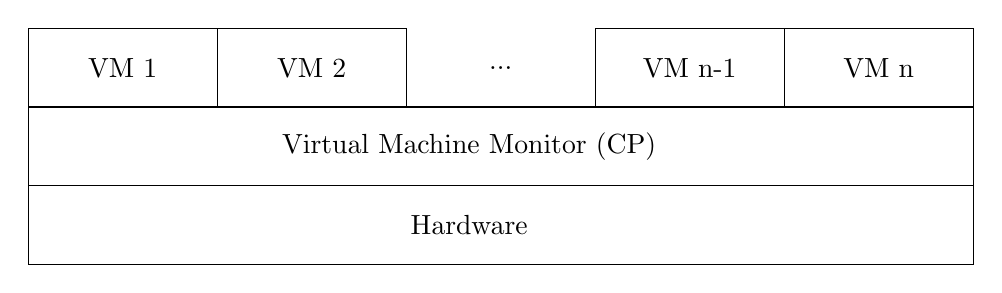
\begin{tikzpicture}[ scale=2, ]
\node[black,shape=rectangle] at (0.6,0.25) {VM 1};
\node[black,shape=rectangle] at (1.8,0.25) {VM 2};
\node[black,shape=rectangle] at (3,0.25) {...};
\node[black,shape=rectangle] at (4.2,0.25) {VM n-1};
\node[black,shape=rectangle] at (5.4,0.25) {VM n};

\node[black,shape=rectangle] at (2.8,-.25) {Virtual Machine Monitor (CP)};
\node[black,shape=rectangle] at (2.8,-.75) {Hardware};

\draw (0,0) rectangle (1.2,0.5);
\draw (1.2,0) rectangle (2.4,0.5);
\draw (3.6,0) rectangle (4.8,0.5);
\draw (4.8,0) rectangle (6,0.5);

\draw (0,0) rectangle (6,-.5);

\draw (0,-.5) rectangle (6,-1);


\end{tikzpicture}
\end{center}